%%%%%%%%%%%%%%%%%%%%%%%%%%%%%%%%%%%%%%%%%%%%%%%%%%%%%%%%%%%%%%%%%%%%%%%%%%%%%%%
%%
%% FACHHOCHSCHULE SALZBURG GMBH
%% Informationstechnik und System-Management
%%
%% Salzburg University of Applied Sciences
%% Information Technologies and Systems Management
%%
%%%%%%%%%%%%%%%%%%%%%%%%%%%%%%%%%%%%%%%%%%%%%%%%%%%%%%%%%%%%%%%%%%%%%%%%%%%%%%%
%%
%% Bachelor Thesis 1
%% Aufbau eines Mobile IPv6 Szenarios im Netzwerklabor
%% LaTeX template
%%
%% Theoretischer Teil
%%
%% Riccardo Martin, Michael Pfn�r, Daniel Zotter
%%%%%%%%%%%%%%%%%%%%%%%%%%%%%%%%%%%%%%%%%%%%%%%%%%%%%%%%%%%%%%%%%%%%%%%%%%%%%%%


\chapter{Theoretischer Teil}
\label{chapter_grundlagen}

%Der Kernteil der Arbeit beginnt mit einer Darstellung der Grundlagen. Dieser, in der Regel rein theoretische Abschnitt, beinhaltet Begriffsbestimmungen, Beschreibungen zur Methodik und zum verwendeten Material, zu Hard- und Software sowie Begriffsabgrenzungen und anderweitigen Grundlagen ("`Material und Methode"'), welche zum Verst�ndnis der nachfolgenden Ausf�hrungen notwendig sind.
Mobile IPv6 ist ein Protokoll, dass von der IETF entwickelt wurden welches es erm�glicht, eine feste IPv6 Adresse einem mobilen Endger�t zuzuweisen und diese auch bei Netzwechseln zu behalten.  
Im folgenden Kapitel wird auf die theoretische Funktionsweise von \textbf{Mobile IPv6} eingegangen, sowie den Unterschied zwischen den Versionen IPv4 und IPv6. In diesem Teil werden einige Fachbegriffe in Bezug auf Mobile IPv6 verwendet, welche f�r das Verst�ndnis der Funktionsweise wichtig sind. Diese Begriffe werden in Abschnitt \ref{subsection_Begriffserklaerung_MobileIPV6} kurz erkl�rt\cite{RFC_Mobile_IPv6}. 
\section{Mobile IPv6}
\label{section_Mobile_IPv6}
\subsection{Begriffsdefinition}
\label{subsection_Begriffserklaerung_MobileIPV6}

\subsection*{Home Adresse}
Die \textit{Home Adresse} ist eine Unicast Adresse welche dem Mobilen Knoten zugewiesen wird, sie wird als permanente Adresse dieses Knoten benutzt. Diese befindet sich innerhalb des Home Links des mobilen Knoten. IP Routing Mechanismen schicken an die Home Adresse gerichtete Pakete an den Home Link. Falls es mehrere Pr�fixe auf dem Home Link gibt, kann ein Mobiler Knoten auch mehrere Home Adressen besitzen.

\subsection*{Home Subnetz Pr�fix}
Unter \textit{Home Subnetz Pr�fix} versteht man das IP-Subnetzpr�fix, dass der Home Adresse des mobilen Knoten entspricht.

\subsection*{Home Link}
Der \textit{Home Link}, ist der Link an welchem das Home-Subnetzpr�fix definiert ist.

\subsection*{Mobiler node}
Ein \textit{Mobiler node} ist ein Knoten, welcher seinen Standort wechseln kann (z.B. Laptop, Mobil Telefon etc.). Dieser Knoten bleibt aber auch unter seiner Home Adresse erreichbar, wenn er von seinem \textit{Heimnetz A} in ein \textit{Fremdnetz B} wechselt.

\subsection*{Correspondent node}
Ein \textit{Correspondent node} ist ein peer (gleichberechtigter Teilnehmer) Knoten mit dem der mobile Knoten kommuniziert. Der correspondant node kann ein mobiler oder station�rer Knoten sein.

\subsection*{Foreign Subnet Pr�fix}
Unter \textit{Foreign Subnet Pr�fix} versteht man jedes Subnet Pr�fix, das nicht dem Home Subnet Pr�fix des mobilen Knotens entspricht.

\subsection*{Foreign Link}
Ist jeder Link, der nicht dem Home Link des mobilen Knotens entspricht.

\subsection*{Care-of Adresse}
Die \textit{Care-of Adresse} ist eine Unicast Adresse, die dem mobilen Knoten in einem fremden Netz zugewiesen wird. Ein mobiler Knoten kann auch mehrere Care-of Adressen besitzen (z.B. mit verschiedenen Pr�fixes), die Care-of Adresse mit der er bei seinem \textit{Home Agent} registriert ist, wird als \textit{\glqq Primary\grqq Care-of Adresse} bezeichnet.

\subsection*{Home Agent}
Als \textit{Home Agent} wird der Router bezeichnet der sich am \textit{Home Link} des mobilen Knotens befindet und wo die aktuelle \textit{Care-of Adresse} des mobilen Knoten registriert ist. Wenn sich der mobile Knoten nicht im Heimnetz befindet, f�ngt der \textit{Home Agent} die Pakete, die an die Home Adresse des mobilen Knoten im Heimnetz gerichtet sind ab, \glqq verpackt\grqq diese und sendet sie �ber einen Tunnel an die registrierte \textit{Care-of Adresse} des mobilen Knoten.

\subsection*{Binding}
Als \textit{Binding} versteht man die Zuordnung der \textit{Home Adresse} des mobilen Knotens, der \textit{Care-of Adresse} des mobilen Knotens f�r die noch verbleibende lifetime.

\subsection*{Registrierung}
Unter \textit{Registrierung} versteht man, wenn ein Binding Update von einem mobilen Knoten an seinen Home Agent oder an einen Corresponding Node  geschickt und von diesen registriert wird.

\subsection*{Binding Authentisierung}
Damit ein Corresponding Node weiss, dass ein Absender berechtigt ist das Binding zu �ndern, muss eine Registrierung bei einem Corresponding Node autorisiert werden.\newpage

\subsection{Mobility Header}
\label{subsection_Mobility_Header}
F�r das \textit{Mobile IPv6 Protokoll} wurde ein extra \textit{Mobility Header} eingef�hrt. Dieser ist ein \textit{Extention Header}, der von \textit{Correspondig Nodes, mobilen Knoten} und \textit{Home Agents} genutzt wird. Er kommt in allen Nachrichten, die mit dem Herstellen und Verwalten von Bindings zu tun haben vor.\\
Das Format des Mobility Headers ist in Abbildung \ref{Abb_Format_Mobility_Header} dargestellt\cite{RFC_Mobile_IPv6}.

\begin{figure}[h] 
  \centering
     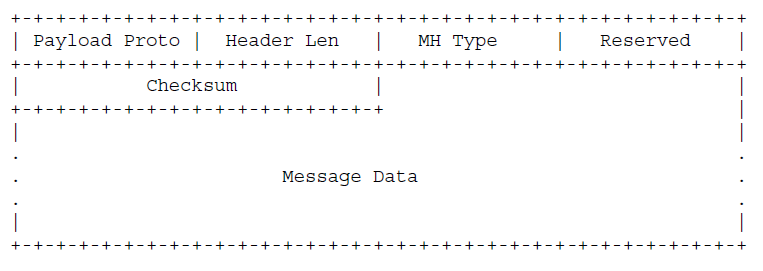
\includegraphics[scale=0.8]{BilderTheoretischerTeil/FormatMobilityHeader.png}
  \caption{Format Mobility Header}
  \label{Abb_Format_Mobility_Header}
\end{figure}

Die im Header definierten Felder haben folgende Aufgabe.

\begin{table}[!h]
%\rowcolors{2}{black!10}{black!20}
\centering
\begin{tabular}{
lll
}

\multicolumn{1}{p{3,5cm}}{\centering \textit{Feld}} & \multicolumn{1}{p{2cm}}{\centering \textit{Gr��e} } & \multicolumn{1}{p{6,5cm}}{\centering \textit{Beschreibung} }\\\midrule
\textbf{Payload Proto} &1\,Byte  & Entspricht dem next Header Feld\\
&&\\
\textbf{Header Len} & 1 Byte & L�nge des Mobility Header\\
&&\\
\textbf{MH Type} & 1 Byte & Identifiziert die betreffende Mobility Nachricht\\
&&siehe Tabelle\\
&&\\
\textbf{Reserved} & 1 Byte & Reserviert f�r zuk�nftige Benutzungen. Der Wert\\
&&\texttt{MUSS} mit 0 von Sender initialisiert werden und \\
&&\texttt{MUSS} vom Empf�nger ignoriert werden\\
&&\\
\textbf{Checksum} & 1 Byte & Enth�lt die Checksum vom Mobility Header\\
&&\\
\textbf{Data} & variabel & Enth�lt die Daten entsprechend des MH Type\\
\bottomrule
\end{tabular}
\caption{Beschreibung Mobility Header Felder}
\end{table}
\label{Tabelle_Mobility_Header_Felder}
\newpage

Im Folgenden werden die verschiedenen \textit{Mobility Nachrichtentypen} aufgezeigt um den Ablauf in einem \textit{Mobile IPv6 Szenario} richtig zu verstehen.

\begin{table}[!h]
%\rowcolors{2}{black!10}{black!20}

\begin{tabular}{
cll
}

\multicolumn{1}{p{1.3cm}}{\centering \textit{MH Wert}} & \multicolumn{1}{p{3.9cm}}{\centering \textit{Nachricht} } & \multicolumn{1}{p{9cm}}{\centering \textit{Beschreibung} }\\\midrule
0 & Binding Refresh  & Fordert den mobilen Knoten auf, sein Binding zu \\
&Request &aktualisieren. Wird vom CN�s verschickt\\
&&\\
1 & Home Test & Eine vom mobilen Knoten verschickte Nachricht um\\
&Init&einen Return routability Prozess zu initialisieren und\\
&&einen Home keygen token vom CN zu erhalten. Diese\\
&&Nachricht ist getunnelt durch den Home Agent, wenn\\
&&sich der mobile Knoten nicht zu Hause befindet.\\
&&\\
2& Care-of Test & Wie \textit{Home Test Init}, nur wird die Nachricht direkt an\\
&Init&den CN geschickt.\\
&&\\
3 & Home Test & Antwort auf \textit{Home Test Init}. Wird vom CN an den\\
&Message & mobilen Knoten gesendet.\\
&&\\
4 & Care-of Test & Antwort auf \textit{Care-of Test Init}. Wird vom CN an den\\
& Message & mobilen Knoten gesendet.\\
&&\\
5 & Binding Update & Wird von einem mobilen Knoten verwendet um \\
& Message & andern Knoten seine neue CoA mitzuteilen\\
&&\\
6 & Binding & Wird verwendet um den Empfang eine Binding\\
&Acknowledgement & Updates zu best�tigen.\\
& Message & \\
&&\\
7 & Binding Error & Wird vom CN verwendet um einen Fehler in Bezug \\
&&auf Mobility zu signalisieren.\\
\bottomrule
\end{tabular}
\caption{Mobility Nachrichtentypen}
\end{table}
\label{Tabelle_Mobility_Nachrichtentypen}

Weiterhin wurde f�r Mobile IPv6 ein neuer Routing Header definiert, der als \textit{Routing Header Type 2} bezeichnet wird. Dieser erlaubt es Pakete direkt von einen CN an die CoA eines mobilen Knoten zu senden. 
\newpage
\subsection{Funktionsweise}
F�r den Ablauf von Mobile IPv6 gibt es zwei verschiedene M�glichkeiten, einmal das \textit{Bidirectional Tunneling} Verfahren und zum Anderen das \textit{Route Optimization} Verfahren.
\subsubsection{Neighbor Discovery}
\subsection*{Bidirectional Tunneling}
Beim Bidirectional Tunneling sind der mobile Knoten und der Home Agent �ber einen Tunnel miteinander verbunden. Pakete die von einem Correspondent Node an einen mobil Node gesendet werden, passieren vor der Zustellung den entsprechenden Home Agent des Mobile Nodes. Alle Pakete die an den mobile Node addressiert sind werden durch den Home Agent abgefangen. Dies geschieht durch \textit{Proxy Neighbor Discovery}. Wenn sich der mobile Node nicht im Heimnetz aufh�lt, werden die vom CN an ihm gesendeten Pakete vom HA verpackt. Alle erkannten Pakete werden an die beim Home Agent in ein neues Paket verpackt, an die registrierte CoA des mobile Node adressiert und �ber den Tunnel gesendet. Am anderen Ende werden die Pakete vom Netzwerk Layer des MN entpackt bevor diese an die oberen Layer weitergegeben werden.\\
�hnlich l�uft es ab wenn der MN Pakete sendet. Hier werden den verpackten Paketen 40\,Byte als Tunnel Header hinzugef�gt und unter Verwendung der CoA des MN an den HA �ber den Tunnel gesendet. Dies wird als \textit{reverse tunneling} bezeichnet. Beim HA werden die Pakete entpackt, der Tunnel Header entfernt und die modifizierten Pakete durch das Internet an den entsprechenden CN gesendet. In Abbildung ist der Ablauf grafisch dargestellt.\cite{Packet_Overhead}
 
\begin{figure}[h] 
  \centering
     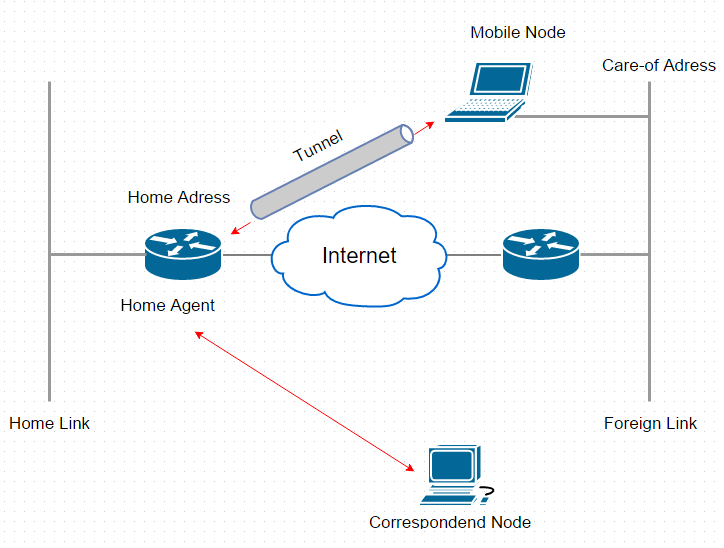
\includegraphics[scale=0.5]{BilderTheoretischerTeil/Bidirectional_Tunnel.png}
  \caption{Bidirectional Tunneling}
  \label{Abb_Bidirectional_Tunneling}
\end{figure}



%\section{Vergleich Mobile IPv4 zu Mobile IPv6}









